\documentclass[12pt]{article}
\usepackage{amsmath}
\usepackage{graphicx}
\usepackage{hyperref}
\graphicspath{ {./resources/} }

\usepackage[T1]{fontenc}
\usepackage[utf8]{inputenc}

\title{Scientific Computing - Condition and Stability}
\author{Mateusz Pełechaty}
\date{23 October 2022}%
\begin{document}
\maketitle
\section*{Exercise 1}
Repeat exercise 5 from previous assignment list, but delete last $9$ in $x_4$ and last $7$ in $x_5$. What influence does it have on the results?
\subsection*{Solution and results}
Previously 
\begin{align*}
x &= [2.718281828, -3.141592654, 1.414213562, 0.5772156649, 0.3010299957]\\
y &= [1486.2497, 878366.9879, -22.37492, 4773714.647, 0.000185049]
\end{align*}
As stated in assignment, we will use 
\begin{align*}
x' = [2.718281828, -3.141592654, 1.414213562, 0.577215664, 0.301029995]
\end{align*}

\begin{table}[!ht]
    \centering
    \begin{tabular}{|l|l|l|l|l|}
    \hline
        ~ & Float32 $x$ & Float32 $x'$ & Float64 $x$ & Float64 $x'$ \\ \hline
        Front & -0.4999 & -0.4999 & 1.025e-10 & -4.296e-3 \\ \hline
        Back & -0.4543 & -0.4543 & -1.564e-10 & -4.296e-3 \\ \hline
        Big To Small & -0.5 & -0.5 & 0.0 & -4.296e-3 \\ \hline
        Small to Big & -0.5 & -0.5 & 0.0 & -4.296e-3 \\ \hline
    \end{tabular}
\end{table}
\subsection*{Conclusions}
As we can see small changes in data completely changes solution

\section*{Exercise 2}
\subsubsection*{Draw graph of $f(x) = e^x ln(1+e^{-x})$ in any two graphing tools. }
\textbf{Desmos}\\
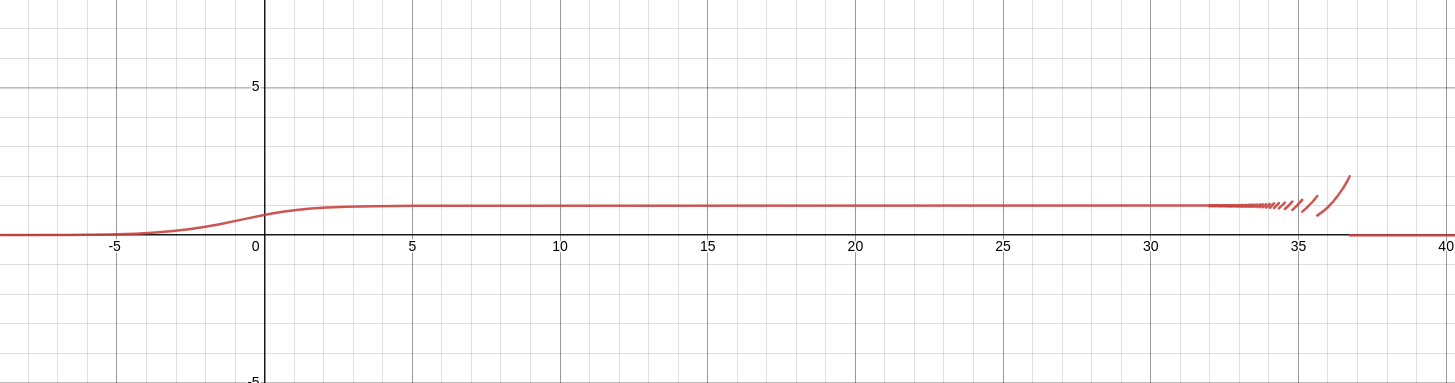
\includegraphics[scale=0.25]{ex2/desmos}\\
\textbf{Geogebra}\\
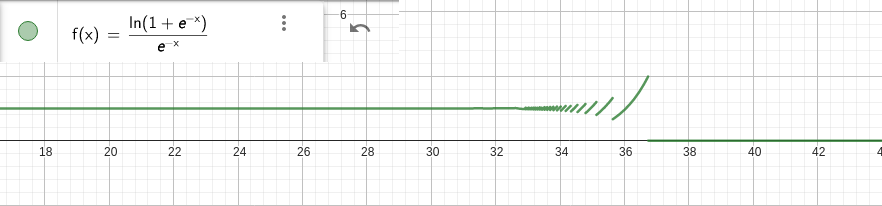
\includegraphics[scale=0.5]{ex2/geogebra}\\
As we can see, Around $x=35$ something happens and $f(x) = 0$ for $x \geq 35$
\subsubsection*{Calculate $\lim_{x->\infty} f(x)$}
$$lim_{x->\infty}f(x) = lim_{x->\infty} e^xln(1+e^{-x}) = lim_{x->\infty} \frac{ln(1+e^{-x})}{e^{-x}} = (\star)$$
Note that $$lim_{x->\infty} ln(1+e^{-x}) = lim_{x->\infty} e^{-x} = 0$$
Because of it we can use L'Hôpital's rule.  
Let's calculate derivatives.
\begin{align*} 
\frac{d}{dx}ln(1+e^{-x}) &= \frac{-e^{-x}}{1+e^{-x}} = \frac{-1}{e^x + 1} \\
\frac{d}{dx}e^{-x} &= -e^{-x}
\end{align*} 
With this we can continue
$$(\star) = lim_{x->\infty} \frac{-1}{e^x + 1} \cdot \frac{-1}{e^{-x}} = lim_{x->\infty} \frac{1}{1 + e^{-x}} = \frac{1}{1+0} = 1$$  
So $\lim_{x->\infty} f(x) = 1$
\subsubsection*{Compare differences between results}
LOREM IPSUM
\section*{Exercise 3}
Consider task of solving system of linear equations
\begin{equation*}
    Ax = b
\end{equation*}
$A \in R^{N \times N}$ - Matrix of coefficients\\
$b$ - vector of right sides\\
Consider two methods of generating $A$\\
\textbf{a.} 
$A = H_n$, where $H_n$ is Hilbert's of $n$ degree generated by $A$=hilb(n)\\
\textbf{b.} 
$A = R_n$, where $R_n$ is random matrix of $n$ degree generated 
with given condition $c$ generated by function $A$=matcond($n$, $c$)\\
Vector $b$ is given $b = Ax$, where $x = (1,\dots,1)^T$
\subsubsection*{Solve $Ax = b$ with $x = \frac{b}{A}$}
\subsubsection*{Solve $Ax = b$ with $x = A^{-1} \cdot b$}

\section*{Exercise 4}
In this exercise we will refer to\\ 
$P(x)$ as to Wilkinson's polynomial in it's general form.\\
$p(x)$ as to Wilkinson's polynomial in factorial form\\
\textbf{1.} Use roots function from Polynomials to compute roots of $P(x)$
Compare calculated roots $z_k$ with real ones. Calculate $|P(z_k)|$, $|p(z_k)|$, $|z_k - k|$ and explain discrepancies.\\
\textbf{2.} Conduct Wilkinson's experiment. Swap coeffincients from $-210$ to $-210-2^{-23}$. Explain results
\section*{Exercise 5}
Consider following reccurence equation that represents population growth
\begin{equation}
    p_{n+1} := p_n + rp_n(1-p_n), n \in \{0, 1, 2, \dots\}
\end{equation}
    $r$ - constant\\
    $r(1-p_n)$ - coefficient of population growth\\
    $p_0$ - starting size of population as a percent of maximum population size
\subsection*{Conduct following experiments}
\textbf{1. } Calculate $p_{40}$ for $p_0=0.01$ and $r=3$. 
Then start again with the same data and calculate $p_{10}$. Then let $p'_{10} := round(p_{10}, 3)$ and continue computing till $p'_{40}$.
Compare $p_{40}$ and $p'_{40}$\\
\begin{table}[h]
    \centering
    \begin{tabular}{|l|l|l|l|}
    \hline
        i & p & p' & |difference| \\ \hline
        10 & 0.7229306 & 0.723 & 6.937981e-5 \\ \hline
        11 & 1.3238364 & 1.323813 & 2.348423e-5 \\ \hline
        12 & 0.037716985 & 0.03780961 & 9.262562e-5 \\ \hline
        13 & 0.14660022 & 0.14694974 & 0.00034952164 \\ \hline
        14 & 0.521926 & 0.5230163 & 0.0010902882 \\ \hline
        15 & 1.2704837 & 1.271427 & 0.0009433031 \\ \hline
        \vdots & \vdots & \vdots & \vdots \\ \hline
        36 & 0.95646656 & 1.3233521 & 0.36688554 \\ \hline
        37 & 1.0813814 & 0.03962612 & 1.0417553 \\ \hline
        38 & 0.81736827 & 0.1537938 & 0.66357446 \\ \hline
        39 & 1.2652004 & 0.5442176 & 0.7209828 \\ \hline
        40 & 0.25860548 & 1.288352 & 1.0297465 \\ \hline
    \end{tabular}
\end{table}
\\
As we can see, $p$ and $p'$ diverged completely after few iterations\\
\textbf{2. } Calculate $p_{40}$ for $p_0=0.01$ and $r=3$ in Float32 and Float64. Compare the results

\begin{table}[h]
    \centering
    \begin{tabular}{|l|l|l|l|}
    \hline
        i & $p_i$ Float32 & $p_i$ Float64 & |Float32 - Float64| \\ \hline
        0 & 0.01 & 0.01 & 2.2351741811588166e-10 \\ \hline
        1 & 0.0397 & 0.0397 & 1.4781951912512525e-9 \\ \hline
        2 & 0.15407173 & 0.15407173000000002 & 3.3555221379266698e-9 \\ \hline
        3 & 0.5450726 & 0.5450726260444213 & 1.089778434160138e-8 \\ \hline
        4 & 1.2889781 & 1.2889780011888006 & 9.863419747624391e-8 \\ \hline
        5 & 0.1715188 & 0.17151914210917552 & 3.3946635324966223e-7 \\ \hline
        \vdots & \vdots & \vdots & \vdots \\ \hline
        37 & 1.0813814 & 0.6822410727153098 & 0.39914036744734893 \\ \hline
        38 & 0.81736827 & 1.3326056469620293 & 0.5152373779953545 \\ \hline
        39 & 1.2652004 & 0.0029091569028512065 & 1.262291219607769 \\ \hline
        40 & 0.25860548 & 0.011611238029748606 & 0.24699424216434318 \\ \hline
    \end{tabular}
\end{table}
As we can see, $p_i$ in Float32 and $p_i$ in Float64 started slowly diverging in the beginning, but near $p_{40}$ they were completely diverged 
\section*{Exercise 6}
Consider reccurence equation
\begin{equation*}
    x_{n+1} := x_n^2 + c, n \in \{0, 1, 2, \dots\}
\end{equation*} 
where $c$ - constant\\
For the following data, compute $x_{40}$ and observe behaviour of generated sequences
\begin{table}[!ht]
    \centering
    \begin{tabular}{ccc}
    \hline
        ID & $c$ & $x_0$ \\ \hline
        1 & -2 & 1 \\ 
        2 & -2 & 2 \\ 
        3 & -2 & 1.99999999999999 \\ 
        4 & -1 & 1 \\ 
        5 & -1 & -1 \\ 
        6 & -1 & 0.75 \\ 
        7 & -1 & 0.25 \\ \hline
    \end{tabular}
    \caption{Data to conduct experiment}
\end{table}
\end{document}